Case~5a is a trivial test for loss curve calculation involving a source model consisting of multiple sources. This case assumes importance if the parallelization strategy of the hazard curve calculators is employed. Given that the source model consists of multiple sources, a task for each source can be defined, and therefore the task creation and aggregation of the results can be tested. The two sources comprising the single source model in this case are the ones described in Case~1a and Case~1b respectively. Given a reasonably large stochastic set of events, we should expect the rates of loss exceedance in this case to be the sum of the corresponding rates from Case~1a and Case~1b.

There is no uncertainty in the vulnerability function used for this case. Table~\ref{tab:vf-ln-tax1-zcov} shows the mean loss ratios and corresponding coefficients of variation in the lognormal vulnerability function used in this case.

The loss curve calculated using the implementation of the calculator in Julia is compared with that produced by OpenQuake in Figure~\ref{fig:lc-ebr-5a}.

\begin{figure}[htbp]
\centering
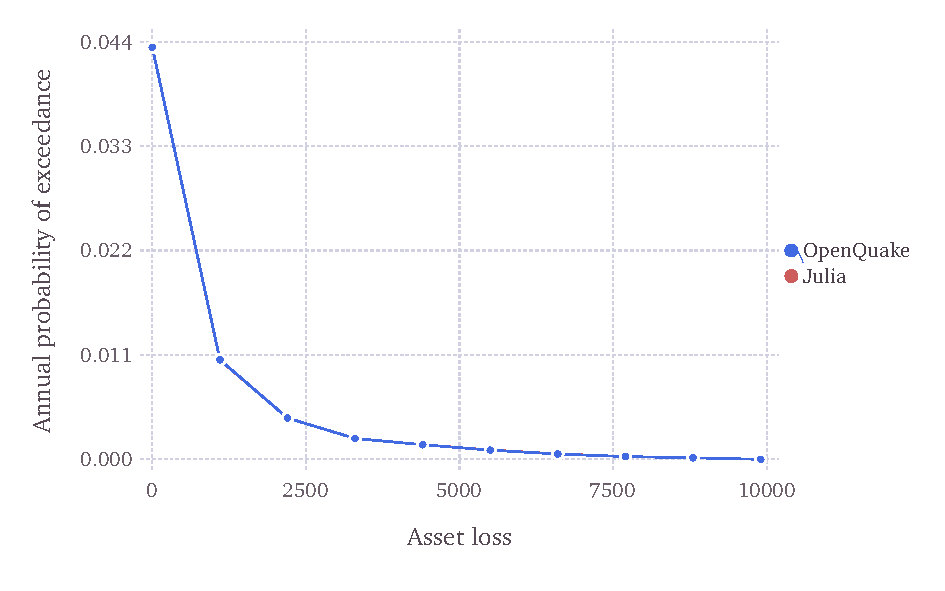
\includegraphics[width=12cm]{qareport/figures/fig-lc-ebr-5a}
\caption{Loss curve comparison for event based risk test case 5a}
\label{fig:lc-ebr-5a}
\end{figure}